\documentclass[Orbiter Developer Manual.tex]{subfiles}
\begin{document}

\section{Orbiter program flow and module callback order}
This section defines the program flow of the Orbiter frame loop and the order in which module callback functions are called by Orbiter.


\subsection{The frame update loop and vessel module callback functions}

The program flow diagram below illustrates the events in the Orbiter frame update loop and the calling order of VESSEL2 callback functions.\\
The clbkPreStep and clbkPostStep methods are called for every vessel at each frame update. Other callback functions are only called when the associated event has occurred. Some callback functions such as clbkPanelRedrawEvent may be called multiple times for a vessel in a single frame.

\begin{figure}[H]
	\centering
	\subfigure{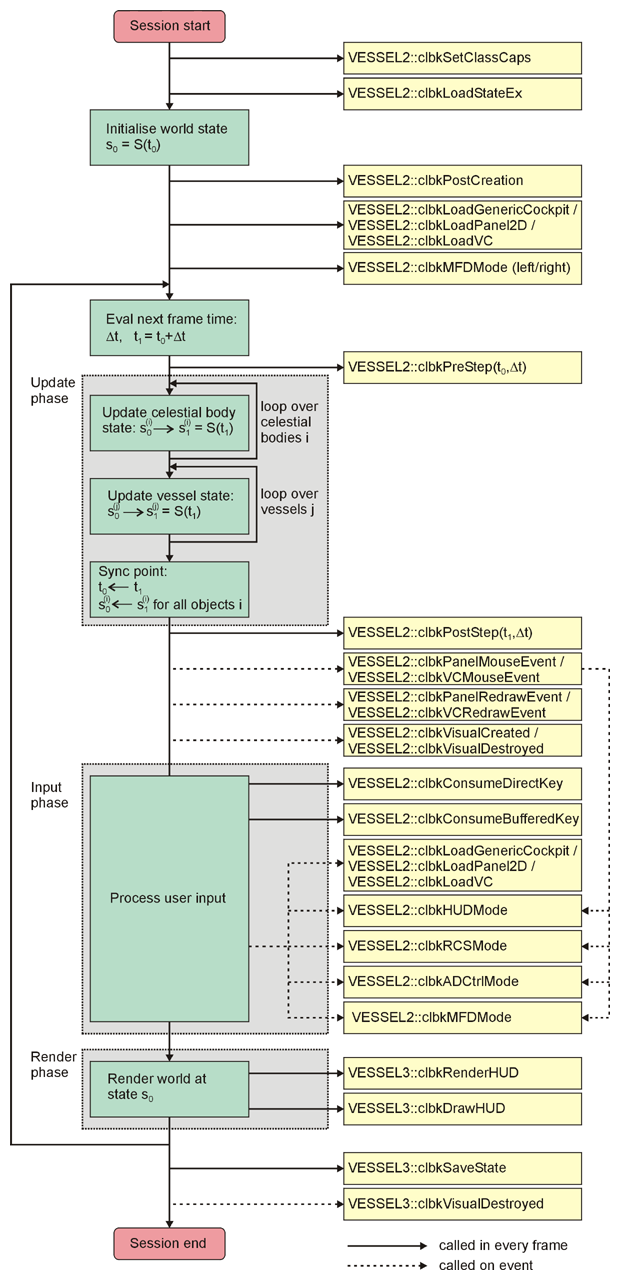
\includegraphics[width=0.65\textwidth]{progflow1.png}}
	\caption{Orbiter frame update loop and position of VESSEL2 callback functions.}
\end{figure}

\end{document}
